

\chapter{Evaluace}\label{kap:evaluace}

V této kapitole popíšeme uživatelské testování a celkovou evaluaci aplikace.

\section{Uživatelské testování}

Uživatelské testování bylo směřováno hlavně na uživatele s rolí veřejnost (viz uživatelské role popsané v části \ref{sec:role}), protože tento typ uživatelů bylo možné pro testování získat.

Testování jsme provedli podle metodiky System Usability Scale (SUS) \footnote{\url{https://www.usability.gov/how-to-and-tools/methods/system-usability-scale.html}}, která se používá ke zhodnocení použitelnosti uživatelských rozhraní aplikací. Uživatelé byli nejdříve seznámeni s účelem a základním fungováním aplikace. Poté měli projít 3 testovací scénáře, které jsou založené na případech užití pro roli veřejnost. Scénáře jsou podrobněji popsané v části \ref{sub:test-cases}. 

Nakonec měli ohodnotit, jak dobře se s aplikací pracuje v 10 standardizovaných otázkách z metodiky SUS. Každá otázka obsahovala tvrzení, na které bylo možné odpovědět jedním z 5 stupni souhlasu od zcela nesouhlasím k určitě souhlasím. Dotazník obsahoval tvrzení jako:
\begin{itemize}
    \item Systém mi přišel příliš složitý.
    \item Systém mi přišel snadno použitelný.
    \item Přišlo mi, že různé funkce tohoto systému jsou dobře integrovány.
    \item Při používání systému jsem se cítil(a) že vím co dělám.
\end{itemize}
Uživatele jsme také požádali o zpětnou vazbu a návrhy na vylepšení aplikace.

\subsection{Testovací scénáře}\label{sub:test-cases}

Uživatelé měli během testování projít 3 testovací scénáře, které jsou založené na případech užití, které patří k roli veřejnost. Na obrázku \ref{fig:use-cases-verejnost} vidíme část diagramu případů užití, kde jsou vybrané pouze ty případy užití, které se týkají uživatelů s rolí veřejnost. Všechny případy užití jsou popsané v části \ref{sec:use-cases}.

\begin{figure} 
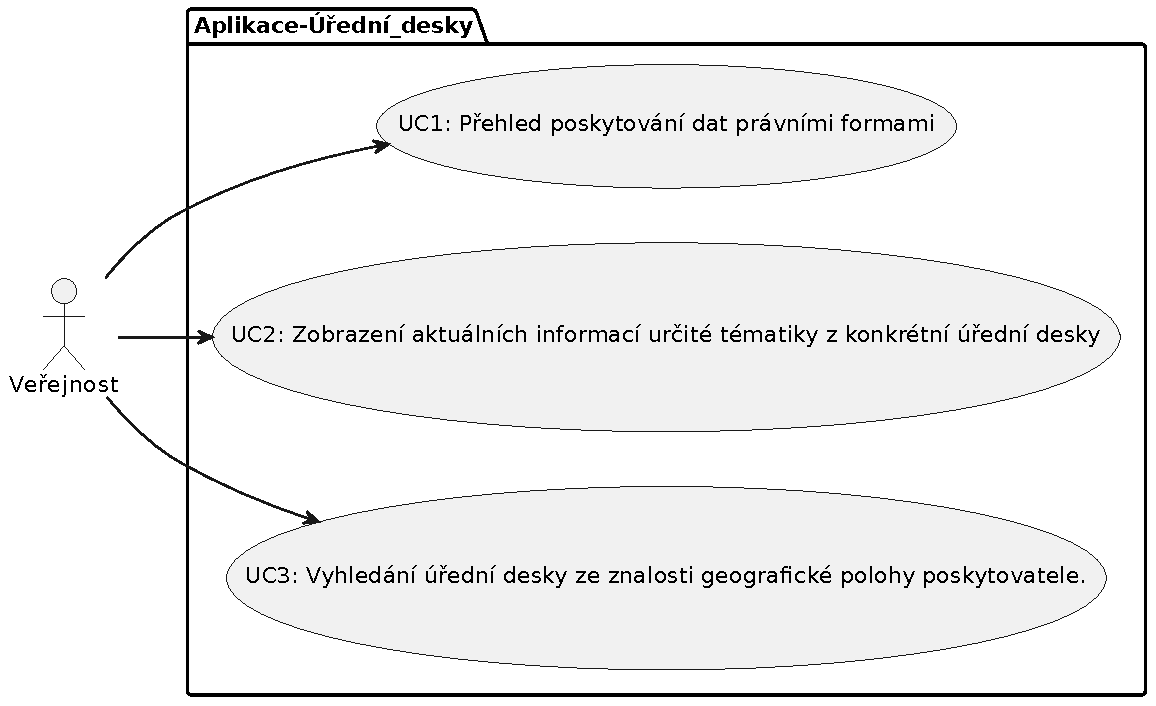
\includegraphics[width=\textwidth]{cs/obrazky/use-case-diagram-verejnost.pdf}
\caption{Diagram případů užití --- veřejnost}
\label{fig:use-cases-verejnost}
\end{figure}

Pro tyto případy užití byly navrženy následující testovací scénáře.

\subsubsection{Zobrazení aktuálních informací určité tématiky z konkrétní úřední desky}

Chceme najít informace, které se týkají dražeb v Městské části Praha 12.
\begin{enumerate}
    \item Otevřete aplikaci z odkazu: 
    \url{https://bliakher.github.io/uredni_desky}. Měla by se otevřít stránka se seznamem všech úředních desek.
    \item Pomocí formuláře pro vyhledávání najděte úřední desku Městské části Praha 12.
    \item Otevřete detail desky kliknutím na tlačítko \textit{Zobrazit informace}.
    \item Nyní byste měli vidět všechny informace vyvěšené na této desce.
    \item Použijte formulář na vyhledávání v informacích k nalezení informací, které se týkají dražeb.
    \item Prohlédněte si informace o dražbách.
\end{enumerate}

\subsubsection{Přehled poskytování dat právními formami}

Chceme zjistit, které krajské úřady poskytují svoji úřední desku.
\begin{enumerate}
    \item V aplikaci se vraťte na seznam úředních desek kliknutím na \textit{Seznam} v navigačním panelu.
    \item Vyfiltrujte pouze ty desky, jejichž poskytovatelem je krajský úřad. To uděláte pomocí panelu \textit{Vyberte právní formu poskytovatele}, kde necháte vybranou pouze právní formu Kraje.
    \item V seznamu by měly zůstat pouze úřední desky krajů.
    \item Prohlédněte si, které kraje poskytují svoji úřední desku.
\end{enumerate}

\subsubsection{Vyhledání úřední desky ze znalosti geografické polohy poskytovatele.}

Chceme najít úřední desky v okolí.
\begin{enumerate}
    \item  V aplikaci přejděte do části s mapou kliknutím na \textit{Mapa} v navigačním panelu.
    \item  Měla by se vám zobrazit mapa ČR, na kterém jsou body vyznačená sídla poskytovatelů úředních desek. Když kliknete na nějaký bod, zobrazí se vám úřední desky daného poskytovatele.
    \item Najděte na mapě obec, ve které bydlíte.
    \item Zjistěte, jestli vaše obec nebo váš krajský úřad poskytuje úřední desku, případně jaké obce v okolí ji poskytují.
\end{enumerate}


\subsection{Výsledky testování}\label{sub:vysledky-testovani}

Testování se zúčastnilo 11 uživatelů. Získali jsme následující výsledky.

Většina uživatelů se shodla na tom, že systém není příliš složitý a naopak je snadno použitelný. Uživatelé při používání systému cítí, že ví, co dělají a nepotřebují podporu technického personálu.

Někteří uživatelé hodnotili systém jako těžkopádný. Na tvrzení: \textit{``Systém mi přišel velice těžkopádný.''} odpovědělo 6 uživatelů \textit{určitě nesouhlasím}, 3 \textit{spíše nesouhlasím} a 2 \textit{spíše souhlasím}.

Několika uživatelům přišla aplikace v něčem nekonzistentní. Na tvrzení: \textit{``Přišlo mi, že je systém příliš nekonzistentní (rozdílné názvy pro stejné věci, rozdílné ovládání podobných prvků...)''} odpovědělo 7 uživatelů \textit{určitě nesouhlasím}, 2 \textit{spíše nesouhlasím}, 1 \textit{nemám názor} a 1 \textit{spíše souhlasím}.

Všechny odpovědi uživatelů v testování shromážděné podle tvrzení je možné najít v tabulce v příloze \ref{fig:testovani-vysledky}. 

Podle metodiky SUS bylo pro každého uživatele vypočítané skóre aplikace. Výsledky je možné najít v příloze \ref{fig:testovani-skore}. Pokud má skóre hodnotu vyšší než 68, můžeme to podle metodiky interpretovat tak, že je aplikace z hlediska použitelnosti lepší než průměrná aplikace. Průměrné skóre aplikace vyšlo 87,05.

Kromě výsledků dotazníku, jsme od uživatelů také získali zpětnou vazbu k aplikaci.

Na doporučení uživatelů byly barevně zvýrazněné některé prvky, které jsou důležité pro navigaci v aplikaci, jako například tlačítko \textit{Zobrazit informace}, které umožňuje přejít ze seznamu do detailu desky. Také bylo přidáno navigační tlačítko \textit{Zpět}, které slouží pro návrat z detailu vizualizace nebo validace zpět do seznamu.

Jako možná vylepšení aplikace uživatelé zmiňovali přidání našeptávání ve formulářích pro vyhledávání.

\section{Evaluace --- poskytovatelé dat}

Aplikaci jsme rozeslali několika představitelům úřadů, které jsou poskytovateli dat z úředních desek. Byl vysvětlen účel a základní fungování aplikace a poskytovatelé dat byli požádáni o zpětnou vazbu k fungování aplikace z jejich pohledu.

Poskytovatelé hodnotili aplikaci pozitivně. Jako možná vylepšení navrhovali v části vizualizace desky rozdělení informací tématicky (např. doprava, výstavba, volby). Toto je teoreticky proveditelné pomocí atributu \texttt{agenda} \footnote{\url{https://ofn.gov.cz/úřední-desky/2021-07-20/\#vazba-informace-agenda}}, který je možné přidat k informaci na úřední desce podle OFN pro úřední desky. Tento atribut ale není mezi doporučenými atributy a ne všichni poskytovatelé ho používají.

V části validace byl návrh na přidání více možností pro filtrování tabulky, které by bylo zabudované do hlavičky tabulky --- mohlo by se jednat například o abecední řazení nebo řazení podle počtu informací na desce. 

